\documentclass{article}

\usepackage[a4paper,left=18mm,right=18mm,top=20mm,bottom=18mm]{geometry}
\usepackage[italian]{babel}

\usepackage{titling}
\usepackage{graphicx}
\usepackage{subcaption}
\usepackage{float}
\usepackage{hyperref}


\title{Breve report sui risultati ottenuti tesi}
\author{David Guzman Piedrahita and Marco Vinciguerra}
 
\begin{document} 
\maketitle        
\section{Introduzione e reti neurali utilizzate}
Per studiare la potenziale relazione tra ammoniaca e particolato in Lombardia, sono state utilizzate
diverse strategie di machine learning al fine di trovare un modello in grado di descrivere 
nel modo più accurato possibile, il comportamento e le interazioni tra le due 
sostanze in questione. 
\\In particolare, sono state utilizzate diverse tipologie di rete neurali LSTM (long-short term memory),
strumenti adatti a modellizzare serie storiche i cui valori dipendono dal passato utilizzando le informazioni degli
istanti temporali precedenti. I diversi modelli implementati permettono di 
gestire dati mancanti nel dataset, e sono in grado
di migliorare il rendimento dei modelli, stabilizzandolo e rimuovendo le informazioni superflue.
    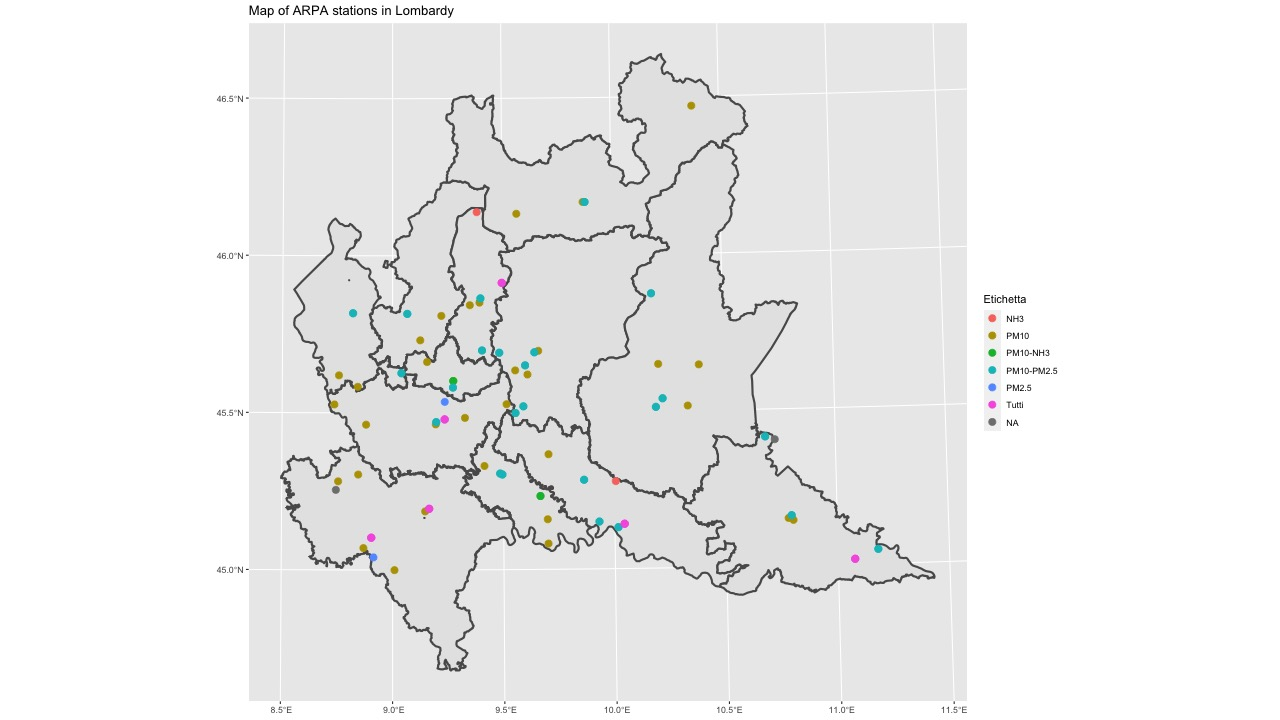
\includegraphics[scale=0.3]{Immagini/mappaTipologie.jpeg}

Il problema dei dati mancanti in questo tipo di analisi riveste un ruolo importante
in quanto i sensori di rilevamento degli inquinanti vengono spesso disattivati causando la perdita 
dei dati. In questo caso, come si può vedere dalla figura seguente, i dati mancanti, sottolienati in blu, sono molto frequenti.
\\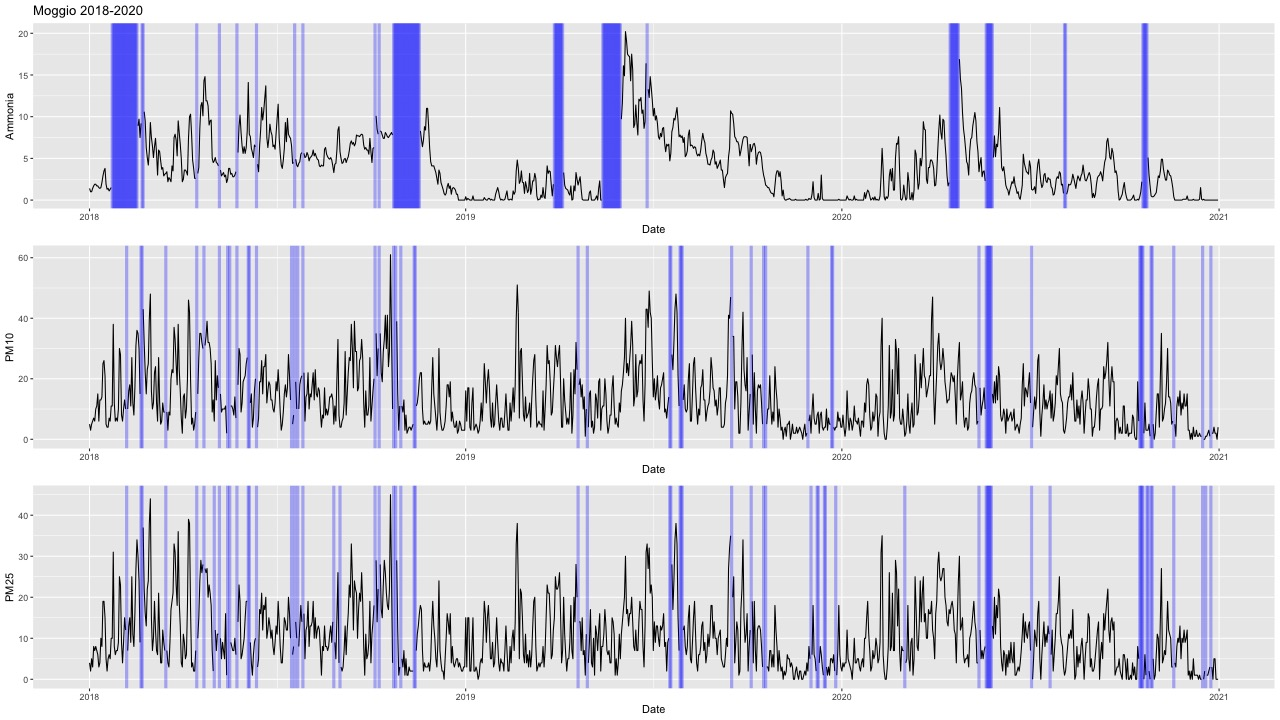
\includegraphics[scale=0.4]{Immagini/Moggio 2018-2020.jpeg}
    
\section{Caso studio e dati}

Le 3 centraline prese in considerazione sono state Moggio, Schivenoglia e 
Cremona via Fatebenefratelli. Le prime 2 sono di tipo rurale mentre l'ultima è di tipo urbano.
Per il caso studio sono stati utilizzati dati provenienti dalle 
tre centraline di qualità dell'aria e da centraline meterologiche dislocate in tutta la Lombardia.
\\Usando, per esempio, i dati della centralina di Moggio dal 2014 al 2020, possiamo ottenere risultati 
che sottolineano una forte relazione tra il particolato e l'ammoninaca, tenendo conto anche di altre variabili
atmosferische, quali: la velocità e la direzione de vento, l'angolatura (tramite il quadrante), la temperatura e le precipitazioni.
\section{Risultati delle reti neurali}
Il dataset a disposizione è stato diviso in training e validazione (scrivere la percentuale)
Infatti,usando per la creazione del mdoelli dati dal 2014 al 2019 e per la 
validazione tutto il 2020. Otteniamo un notevole inseguimento della previsione rispetto ai dati reali, 
usando dati di cinque giorni successivi per determinare l'andamento del sesto giorno.
\section{Regressione tramite reti neurali}
La figura qui sotto rappresenta in arancione il modello da noi ottenuto, 
mentre quello in blu l'andamento reale.
    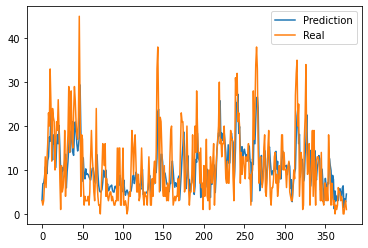
\includegraphics[scale = 0.5]{Immagini/regressionePM25.PNG}

\end{document} 
